\chapter{Implementation and Testing}

This chapter focuses on the implementation stage of this project and discusses the development of the artefact's codebase; the development of this project is dissected into its respected categories, such as each significant chunks of code and overall testing. As stated in section 1, the project will form an executable deliverable which is expected to meet the requirements outlined in \autoref{section:FunctionalRequirements} and \autoref{section:NonFunctionalRequirements} which forms the Minimum Viable Product (MVP) until the final production release. The release of the final deliverable will handled in a staged environment to be assessed.

\section{Linking to Methodology}

This project was developed in an agile manner with continuous development as seen in \autoref{fig:CRISP-DM}, it had one major iteration to which adaptations built into the existing codebase; if test features were needed, a separate git branch was created as insurance the existing (working) code was not affected. The implementation phase is broken down into two key sections as this allows the developer to assess where or not the methodology is functioning as desired with their chosen tech-stack.

\section{Elected Programming Environment}

\subsection{Development Environment}

This project has made use of popular development environments with their own intended purpose:
\begin{itemize}
    \item \textbf{\textit{PyCharm:}} for general development.
    \item \textbf{\textit{Jupyter NoteBooks:}} for data organisation and visualization.
    \item \textbf{\textit{Kaggle NoteBooks}} for open-source testing and comparison.
\end{itemize}

\subsection{Language Choice and Justification}

There are more appropriate languages to consider for this project as the nature is how differing theory implementations affect performance and accuracy; C++ was considered at the beginning of this project due to its performance and execution speeds, popular machine learning libraries are written in C++ such as TensorFlow and ported to Python with the use of Cython. However, the learning curve for writing machine learning in C++ is a lot steeper than in Python to which Python was the chosen language for ease of use and development time.

As the artefact relies on programming knowledge, it was essential to pick a language the developer is comfortable writing in as learning a language for a specific use may have required dedicating too much time, especially with time-management overhead. This was beneficial as the developer has previous experience with Python and is relatively fluent.

As stated above, many a data mining \& analytics and machine learning libraries are written for or in Python which also increases the ease of use for project development with specific traits, such as NLP with ML. This project's interests are heavily backed with open-source development of Python libraries which ensure the imports are relatively low costing and the codebases work as efficiently as possible for a given task. This makes Python a well suited language for machine learning projects and is almost the goto language for data-science related tasks. \newpage

\subsection{Language libraries and Justification}

\begin{itemize}
    \item \textbf{\textit{NLTK:}} Natural Language ToolKit for Python
    \item \textbf{\textit{Pandas:}} Popular Python Library for data-science, particularly, data manipulation and formatting.
    \item \textbf{\textit{Mathlotlib:}} Popular Python library for data visualisation.
\end{itemize}


\section{Data Preparation}

Firstly, the CSV sample data file needs to be cleaned; as the sample data is relatively a small dataset, it can be cleaned manually by simply deleting the unnecessary column headers and values. This was completed within Microsoft Excel by the developer.

\subsection{Data Preprocessing}

Within \autoref{sub:C5Preprocessing}, it states four different data preprocessing methods will be applied, the implementation of those methods are as follows, starting with the removal of punctuation and English stopwords.

\begin{figure}[H]
    \centering
    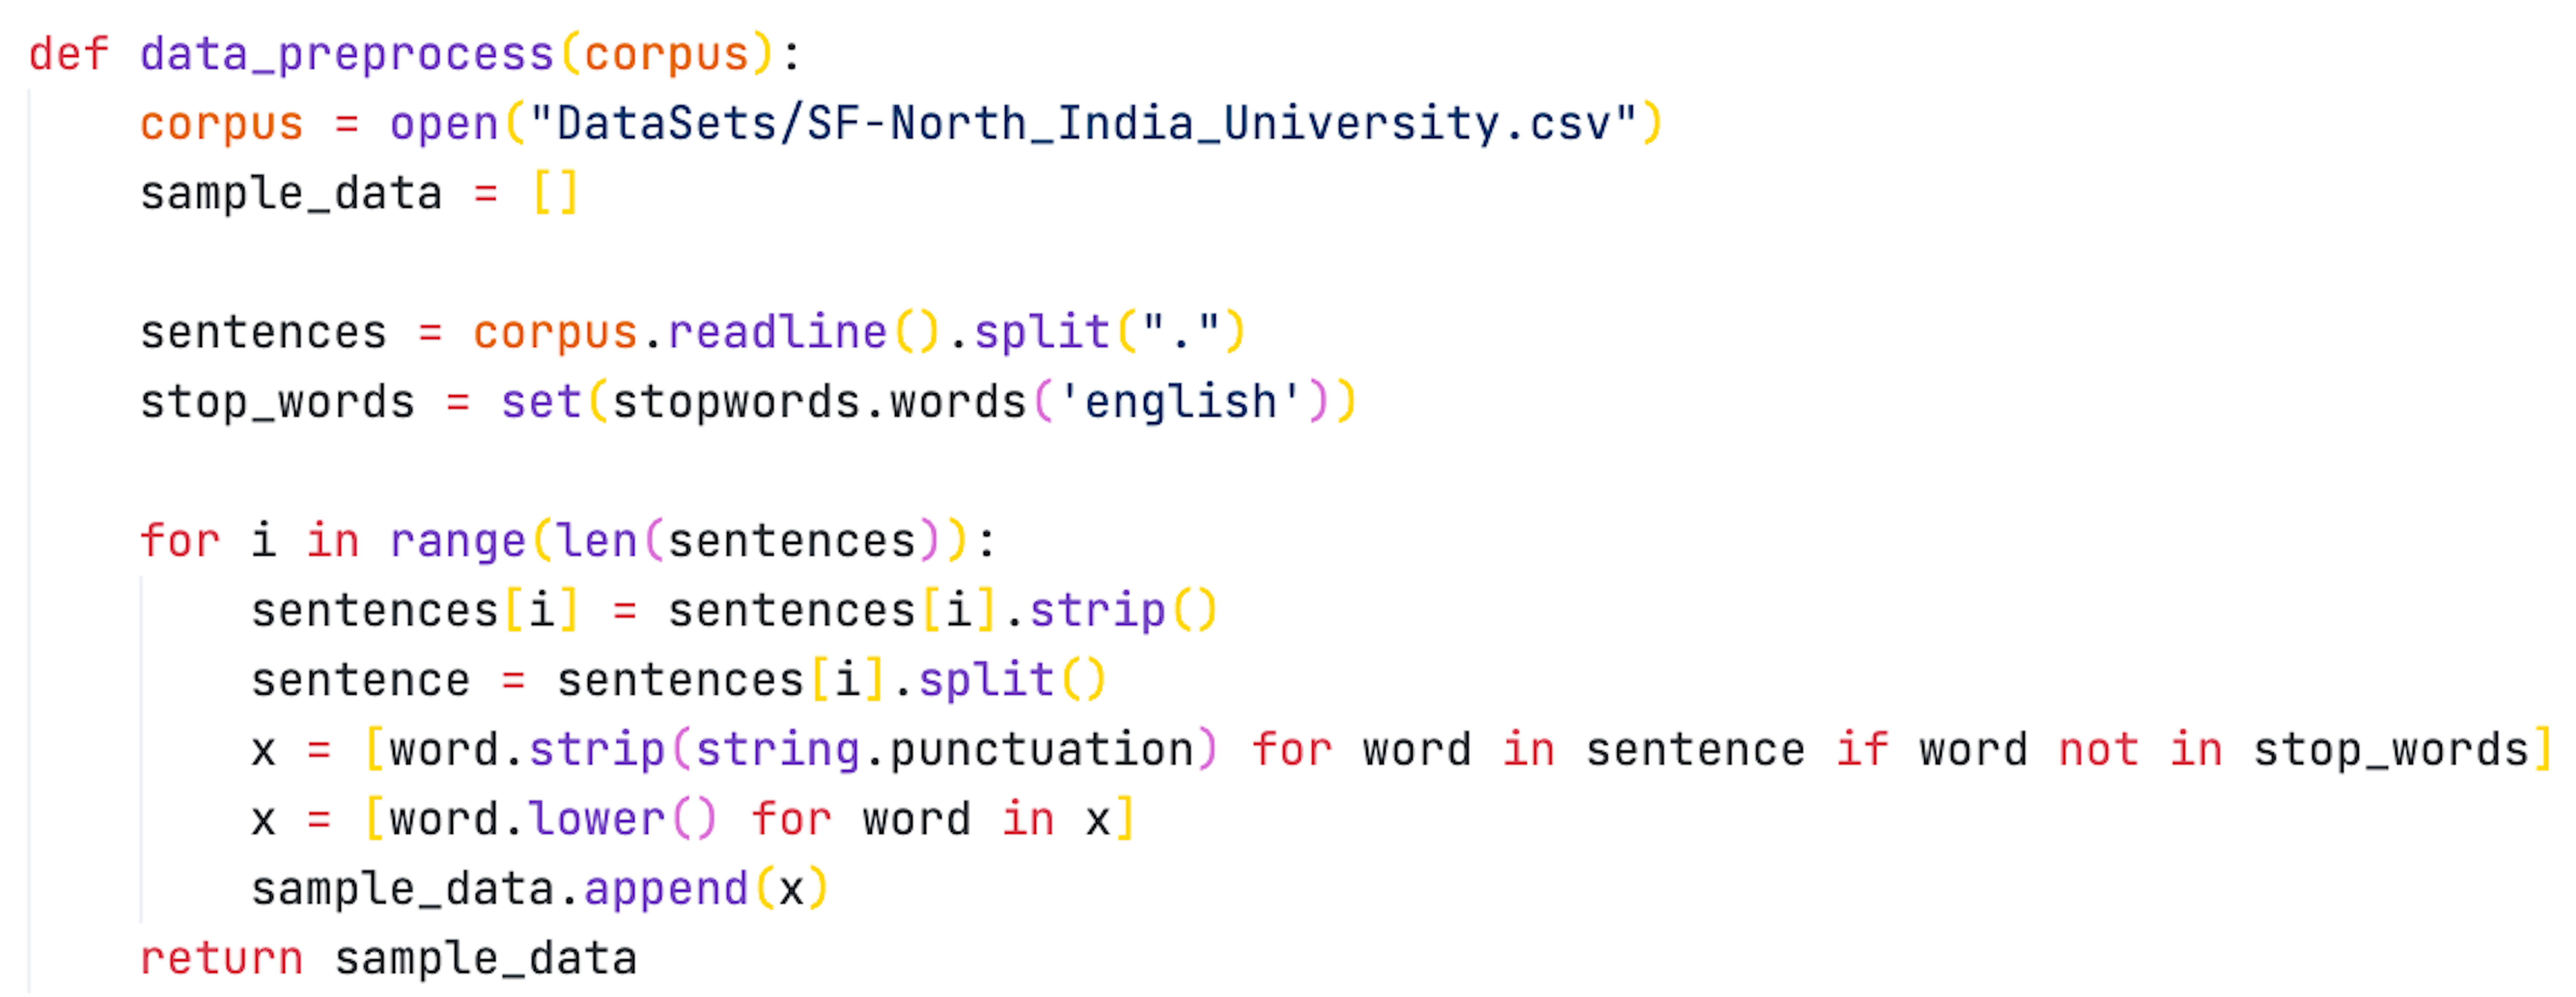
\includegraphics[width=\textwidth]{figures/chapter-6/data_preprocess.png}
    \caption[Code for punctuation and stopword removal on sample data.]{Code for punctuation and stopword removal on sample data.
    \label{fig:data_pre---processing}}
\end{figure}

\newpage

Using pandas, we can apply the functions drop_duplications and isnull to handle colinear values and remove missing values at the same time, this is computational cost effective.

\begin{figure}[H]
    \centering
    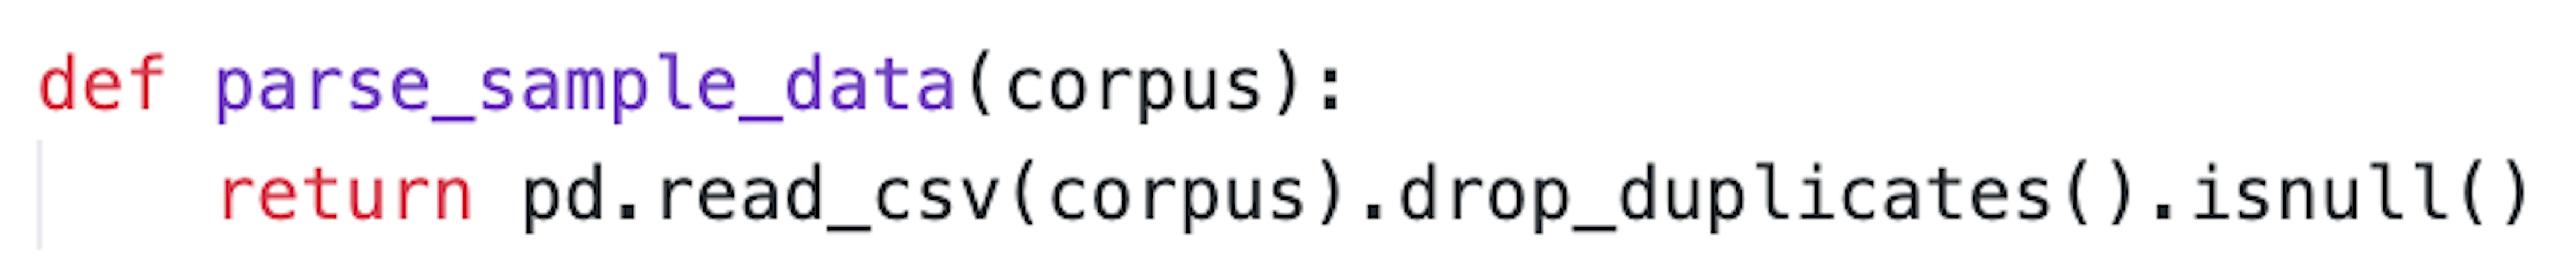
\includegraphics[width=0.8\textwidth]{figures/chapter-6/parse_sample.png}
    \caption[Code for missing and colinear values on sample data.]{Code for missing and colinear values on sample data..
    \label{fig:parse_sample}}
\end{figure}
